\chapter{PELAKSANAAN PENELITIAN}\label{pelaksanaan-penelitian}

%-- NEW SECTION
\section{Alat dan Bahan Penelitian}
Pada Tabel \ref{tab:alat-bahan} ditunjukkan daftar alat dan bahan yang digunakan dalam penelitian ini. \par 
\begin{table}[h!]
    \centering
    \caption{Daftar alat dan bahan yang digunakan dalam penelitian.}
    \begin{tabular}{cp{5cm}p{6cm}}
        \hline
        No. & \multicolumn{1}{c}{Alat dan Bahan}                 & \multicolumn{1}{c}{Spesifikasi}\\
        \hline
        1.  & Laptop MacBook Pro 2015 MF839                      & macOS Big Sur, 2,7 GHz Dual-Core Intel Core i5, RAM 8 GB, Intel Iris Graphics 6100\\
        \hline
        2.  & Visual Studio Code                                 & Versi: 1.62.2\\
        \hline
        3.  & Bahasa Pemrograman Python                          & Versi: 3.9.0\\
        \hline
        4.  & Modul GUI (\textit{Graphical User Interface}) PyQt & Versi: 5.15.4\\
        \hline
        5.  & Qt Designer                                        & Versi: 5.9.6\\
        \hline
        6.  & Data Direktivitas Bundengan                        & Direkam dengan tujuh mikrofon kondensor Behringer ECM8000 \cite{prosidingDirektivitas}\\
        \hline  
    \end{tabular}
    \label{tab:alat-bahan}
\end{table}

%--NEW SECTION
\section{Tata Laksana Penelitian}
Pada Gambar \ref{fig:diagram-alir-penel} ditunjukkan diagram alir dari tata laksana penelitian ini. \par
\begin{figure}[t!]
    \centering
    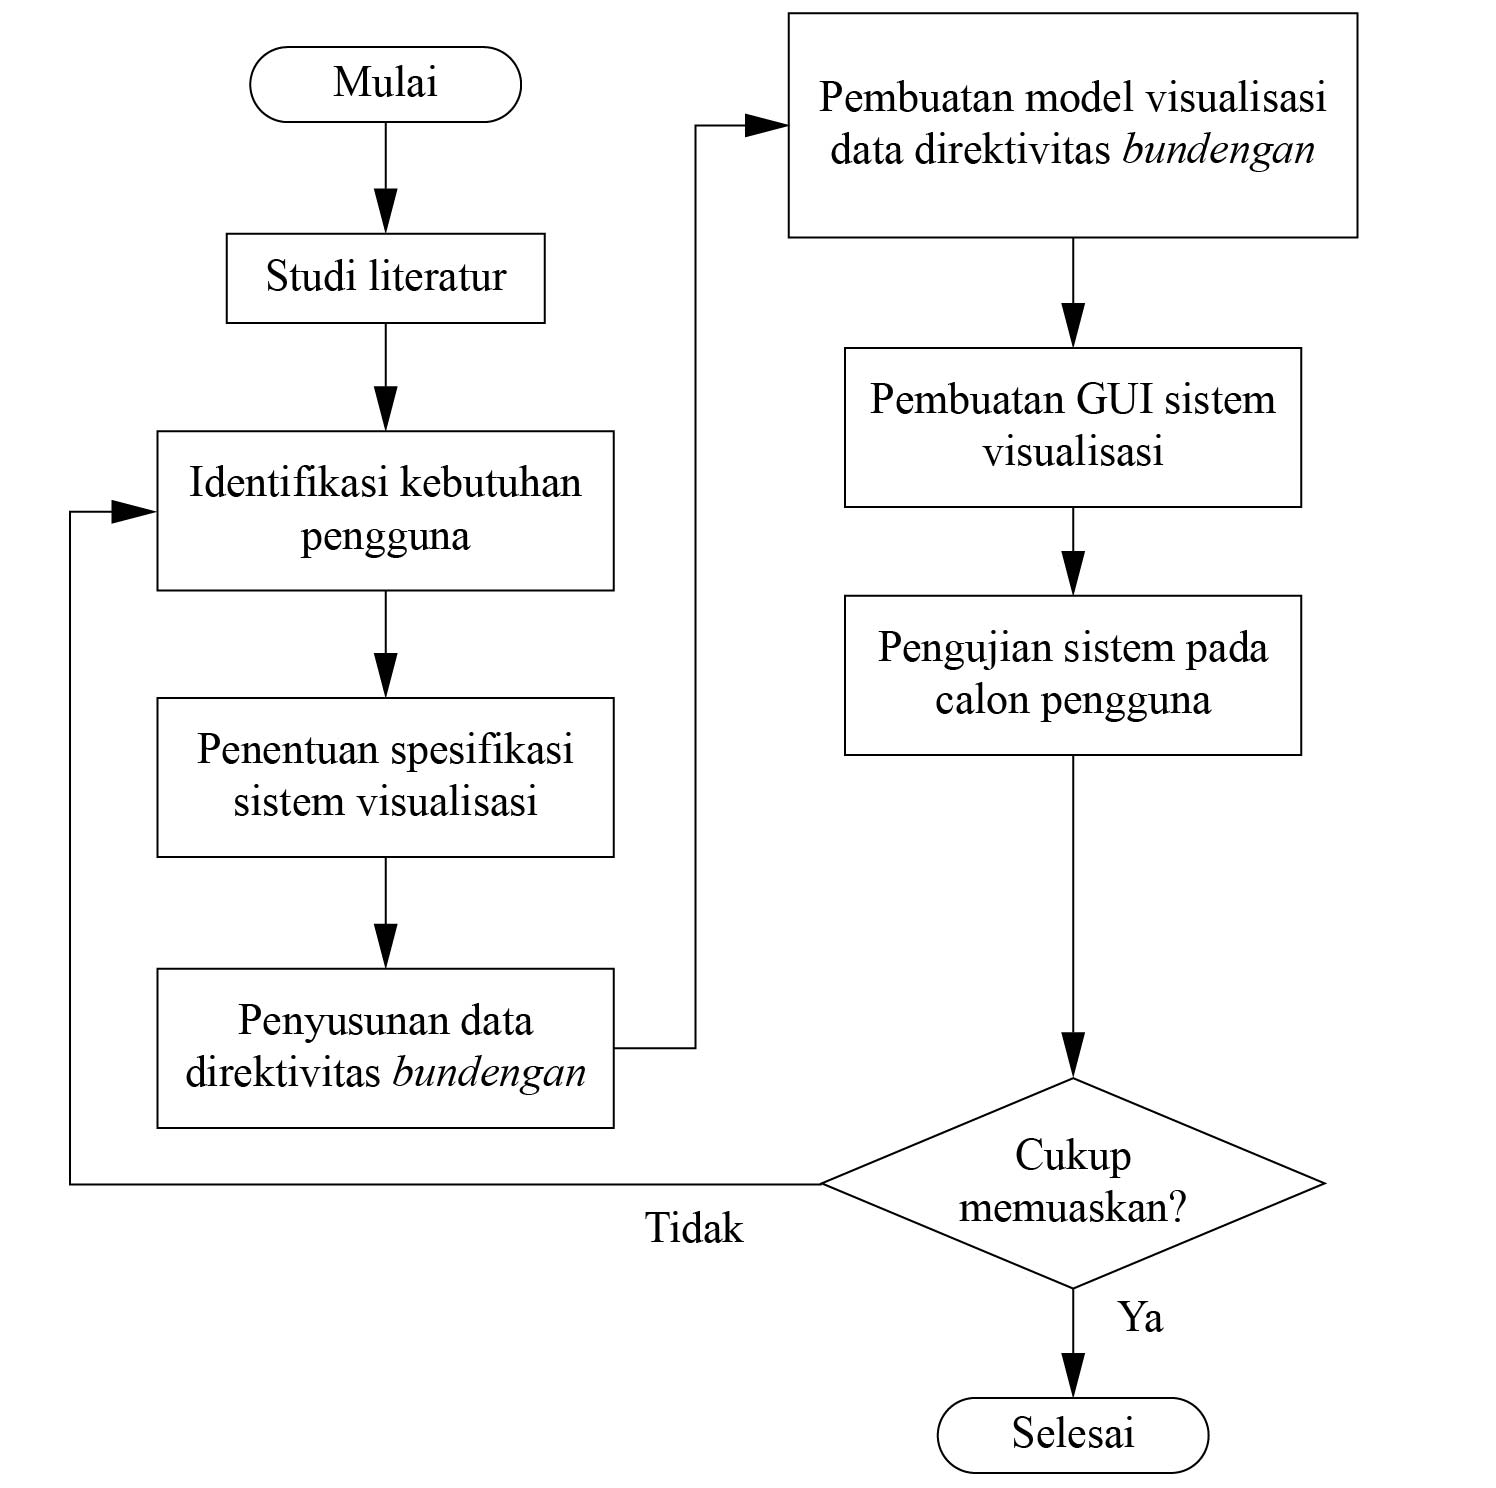
\includegraphics[width=12cm]{Gambar/diagram alir 4_Diagram Alir Bab 4.jpg}
    \caption{Diagram alir tata laksana penelitian.}
    \label{fig:diagram-alir-penel}
\end{figure}
\subsection{Studi Literatur}
Terdapat tiga bagian dalam tahapan studi literatur.
\begin{enumerate}
    \item Pada bagian pertama, dilakukan studi mengenai alat musik \bundengan dan masalah yang sedang dihadapi pemusik \textit{bundengan}. Studi dilanjutkan dengan melakukan tinjauan pustaka terkait perkembangan penelitian yang berkaitan dengan sebaran bunyi yang dihasilkan alat musik \textit{bundengan}. Pemahaman dari tinjauan pustaka kemudian digunakan untuk mempelajari dasar-dasar parameter akustika pada instrumen musik, khususnya alat musik tradisional \textit{bundengan}. Dari studi ini diketahui apa itu \textit{bundengan} dan masalah yang tengah dihadapi, serta parameter akustika pada alat musik \textit{bundengan}.
    \item Pada bagian kedua, dilakukan studi mengenai ilmu yang dibutuhkan untuk penyelesaian masalah yang diketahui pada bagian pertama, yaitu tentang visualisasi data. Selanjutnya dilakukan studi mengenai metode yang dapat ditempuh untuk membangun sistem visualisasi. Dari bagian ini didapatkan pemahaman terkait dasar dan prinsip pada suatu sistem visualisasi dan juga metode paling optimal untuk membangun sistem visualisasi interaktif.
    \item Pada bagian ketiga, dilakukan studi mengenai proses ideal pengembangan produk. Pemahaman pada bagian ini akan dijadikan panduan selama proses perancangan sistem visualisasi. Dari studi ini diketahui bahwa pembuatan sistem visualisasi yang optimal perlu terlebih dahulu mengetahui kebutuhan calon pengguna sehingga dapat menentukan spesifikasi paling optimal dari sistem yang hendak dibangun.
\end{enumerate}
\subsection{Identifikasi Kebutuhan Pengguna}
Tahap ini dimulai dengan pemilihan calon pengguna yang sesuai dengan tujuan sistem visualisasi dibuat, yaitu penyelesaian masalah terkait pementasan musik \textit{bundengan}. Oleh sebab itu, pemilihan calon pengguna didasari oleh beberapa kriteria tertentu. Calon pengguna haruslah orang yang memiliki cukup pengalaman dengan permainan musik \textit{bundengan}, pernah menjadi pengurus atau melakukan pementasan musik \textit{bundengan}, familiar dengan perangkat komputer, dan dapat berkomunikasi dengan keterbatasan kondisi pandemi COVID-19 saat ini. Identifikasi dilakukan melalui wawancara untuk mendapatkan harapan calon pengguna mengenai seperti apa sistem visualisasi ini dapat membantu proses penyelesaian masalah pementasan \textit{bundengan}. Hasil dari tahap ini berupa daftar kebutuhan yang perlu dipenuhi oleh sistem visualisasi. \par 
\subsection{Penentuan Spesifikasi Sistem Visualisasi}
Pada tahap ini dilakukan penentuan rancangan terukur atau spesifikasi dari sistem visualisasi yang dapat memenuhi setiap kebutuhan pengguna. Spesifikasi sistem yang telah ditentukan akan dijadikan panduan ketika membuat model visualisasi dan fitur-fitur yang terdapat pada sistem. Hasil akhir tahap ini berupa daftar spesifikasi sistem yang memenuhi seluruh daftar kebutuhan pengguna pada tahap sebelumnya. \par 
\subsection{Penyusunan Data Direktivitas \Bundengan}
Data direktivitas yang telah diperoleh tersimpan dalam bentuk daftar nilai frekuensi dan TTB untuk setiap arah pada masing-masing senar \textit{bundengan}. Pada tahap ini dilakukan penyusunan arsitektur data direktivitas \bundengan sesuai dengan spesifikasi yang telah ditetapkan. Susunan data ini berhubungan dengan model visualisasi yang akan ditampilkan. Oleh sebab itu, hasil dari tahap ini berupa kode sumber di mana data direktivitas telah disusun sesuai konsep yang direncanakan. \par 
\subsection{Pembuatan Model Visualisasi Data Direktivitas \Bundengan}
Setelah data disusun, tahap selanjutnya adalah memprogram susunan data tersebut menjadi bentuk visual. Teknik visualisasi yang digunakan harus dapat memenuhi kebutuhan pengguna sesuai dengan spesifikasi yang telah ditetapkan. Pembuatan model visualisasi ini dapat dikatakan sebagai inti penelitian karena pada tahap ini dilakukan peningkatan kualitas visual dari tampilan data direktivitas \textit{bundengan} sebelumnya. Hasil akhir dari tahap ini berupa tampilan visual data direktivitas \textit{bundengan}. \par 
\subsection{Pembuatan GUI Sistem Visualisasi}
Berdasarkan Kamus Besar Bahasa Indonesia, interaktif berarti saling melakukan aksi. Suatu sistem interaktif adalah sistem yang saling berkomunikasi dengan pengguna. Untuk mewujudkan hal ini, sistem visualisasi data direktivitas \bundengan perlu dapat menerima masukan dari pengguna berupa perintah atau arahan untuk mencari data, memberi sorotan pada salah satu data, ataupun hal lain sesuai kebutuhan pengguna. Salah satu metode pemberian masukan pada sistem adalah melalui GUI (\textit{Graphical User Interface}). GUI menampilkan antarmuka visual sebagai representasi dari kontroler terhadap sistem \cite{GUI-sumber}. Dengan GUI pengguna dapat melakukan aksi tertentu dan memberi masukan melalui perangkat komputer. Hasil dari tahap ini berupa sistem visualisasi utuh yang siap untuk digunakan. \par 
\subsection{Pengujian Sistem Visualisasi pada Pengguna} 
Setelah sistem visualisasi selesai, selanjutnya sistem akan diuji kinerjanya. Pengujian dilakukan dengan penggunaan sistem visualisasi oleh pengguna kemudian meminta pendapat terkait kualitas sistem tersebut. Hasil dari tahap ini berupa tanggapan penilaian terkait kualitas sistem. Jika respon pengguna setelah uji coba ini mengindikasikan bahwa terdapat kekurangan besar pada sistem maka akan dilakukan perbaikan dan dilakukan uji coba ulang. \par 

%--NEW SECTION
\section{Rencana Analisis Hasil}
Hasil dari penelitian ini berupa sistem visualisasi interaktif data direktivitas \bundengan yang akan digunakan oleh musisi atau pegiat \textit{bundengan}. Analisis akan dilakukan untuk setiap tahapan perancangan dan pembuatan sistem, mulai dari proses identifikasi kebutuhan pengguna sampai dengan sistem selesai dibangun. Selain itu, pada uji kinerja sistem oleh pengguna digunakan SUS sebagai acuan kuantifikasi kualitas sistem. Total skor SUS dijadikan tolak ukur kelayakan sistem visualisasi ini sebagai penyokong penyelesaian masalah pementasan \textit{bundengan}. \par 





